\newsection
\subsection{Adaptation}
\label{sec:adaptation}
\sectionauthors{Xiang Lisa Li*, Eric Mitchell*, Sang Michael Xie, Xuechen Li, Tatsunori Hashimoto}

\begin{figure}[!ht]
\centering
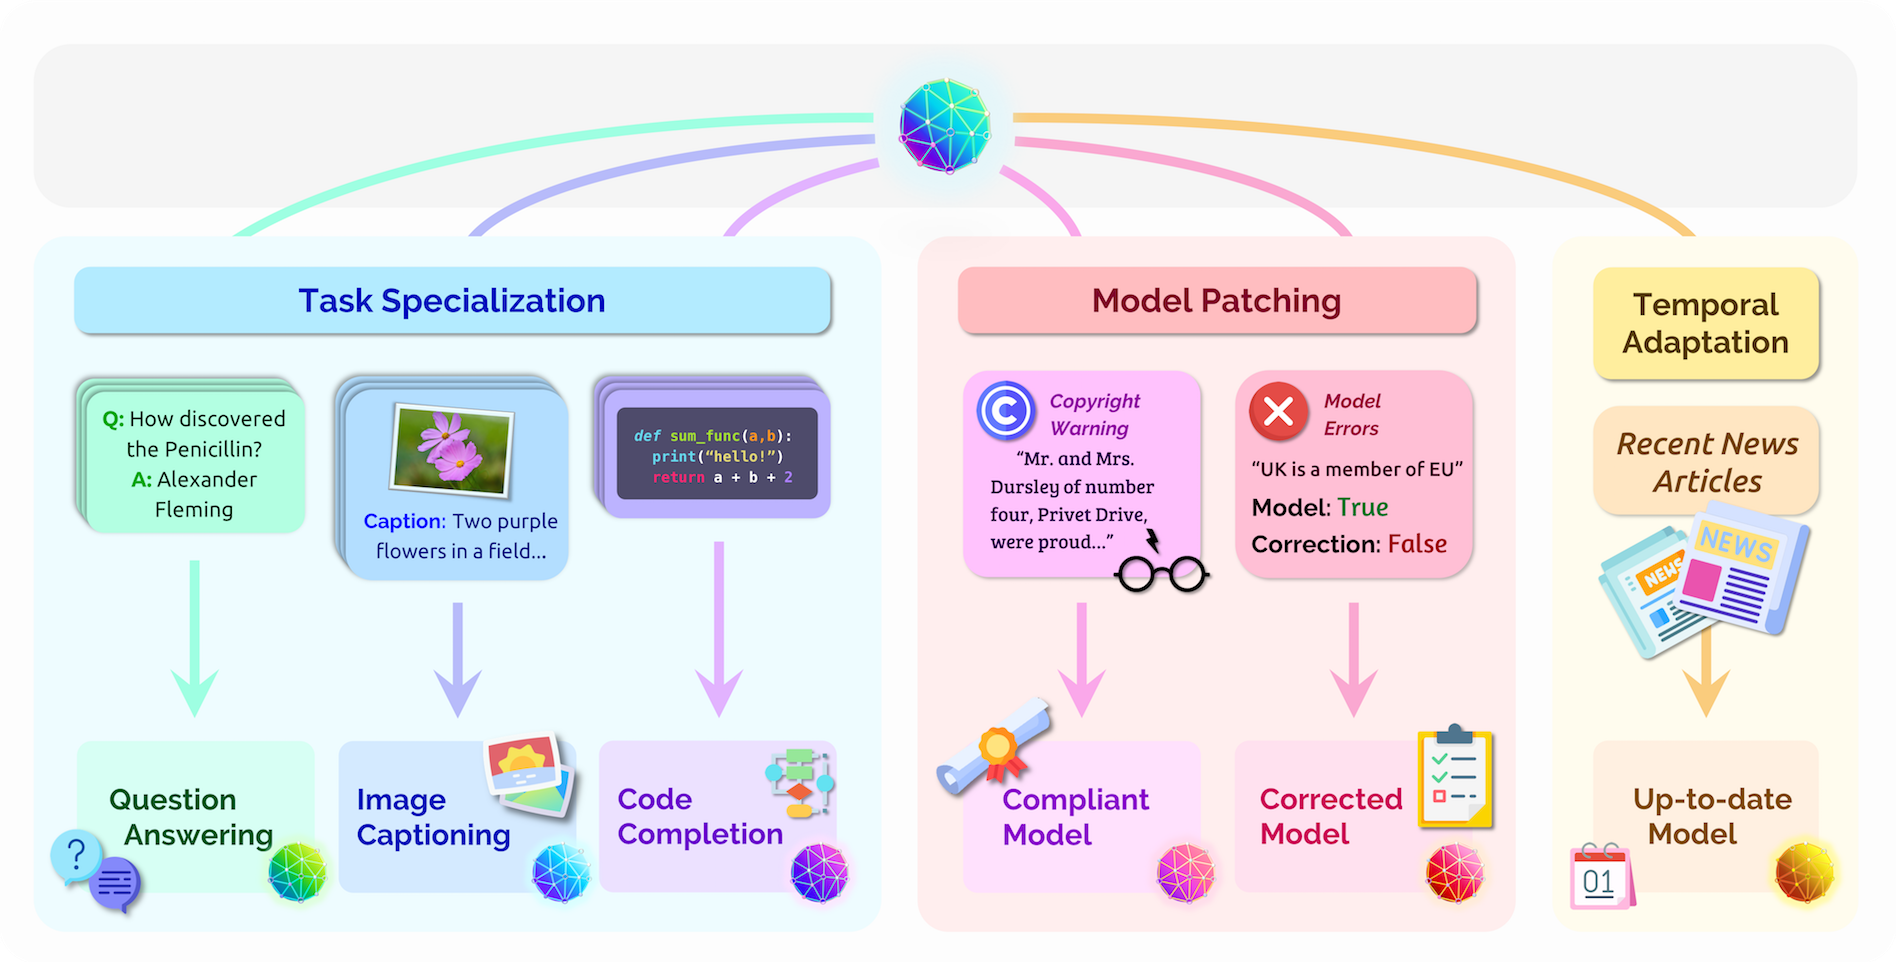
\includegraphics[width=\linewidth]{technology/figures/Adaptation.png}
\caption{\label{fig:adaptation} During adaptation, a foundation model is converted into an \textit{adapted model} (bottom row) in order to reflect updated information, desired behaviors, or deployment constraints.}
\end{figure}

\noindent While foundation models provide a powerful general-purpose engine for processing multi-modal information, \textit{adapting} a foundation model before use is necessary for some applications. Broadly, an adaptation procedure produces an adapted model by conditioning a foundation model on additional information, either by priming the foundation model through the inclusion of new data or a prompt in its input or by updating some or all of the foundation model's parameters to reflect the new information. For example, in text summarization, appending a prompt such as \texttt{TL;DR} to the input article can improve foundation model performance  \citep{radford2019language} by acting as a task specification for the foundation model. Alternatively, fine-tuning the parameters of a foundation model with an organization's internal, domain-specific data could improve the model's accuracy by adding information relevant to the organization’s use case. In this section, we describe existing approaches to adaptation and several factors that determine whether a particular adaptation procedure is appropriate for a particular setting. We additionally describe various use cases for foundation model adaptation, including relatively well-studied settings such as specialization of a foundation model to a particular task or domain as well as more speculative settings like test-time data removal \citep{bourtoule2019machine} and editing model behavior on particular inputs \citep{sinitsin2020editable}. We conclude by presenting a long-horizon goal for future research in foundation model adaptation.
\subsubsection{Methods for foundation model adaptation}
Many methods for adapting foundation models have been proposed, making the decision of \textit{which} adaptation procedure to use for a particular problem or compute environment difficult. We emphasize three factors of particular importance for practitioners to consider when selecting an adaptation procedure: (1) the compute budget (specifically storage and memory); (2) the amount of task-specific data available; and (3) extent of access to foundation model gradients.
\noindent\paragraph{Factor 1: Compute budget.} For foundation models with billions or trillions of parameters, fine-tuning all model parameters may demand prohibitively large memory. Also, separately fine-tuning for many tasks can incur unacceptable storage costs. 
There are many works that propose methods to reduce the storage for adapting foundation models, and we refer to this class of lightweight adaptation methods as \textit{low-storage adaptation}. 
Typically, methods in this class freeze most of the pretrained foundation model parameters and only learn a relatively small number of task-specific parameters (either by fine-tuning some pretrained parameters or by adding altogether new modules), reducing the storage overhead for each task.

The key design decision for such algorithms is the choice of parameters to be adapted. Perhaps the simplest approach is to tune only the final layer of the pretrained model, while other works tune only the model's bias vectors \citep{zaken2021bitfit}, low-rank residuals to model weight tensors \citep{hu2021lora}, or masks over model parameters \citep{zhao2020masking}. Another line of research tunes ``soft'' prompts \citep{li2021prefix,qin-eisner-2021,liu2021prompt, lester2021power,hambardzumyan-etal-2021-warp}, corresponding to sequences of arbitrary parameter vectors rather than embeddings of the model's vocabulary, and conditions the foundation model on these prompts by concatenation with input activations, either at the input layer or at all layers. Another approach freezes all model parameters and interleaves new MLP modules with trainable parameters between existing model layers \citep{houlsby19adapter}. While these lightweight adaptation techniques seem to trade off parameter efficiency and performance on downstream tasks, they sometimes achieve comparable performance to full fine-tuning, despite updating 1000$\times$ fewer parameters \citep{zaken2021bitfit,li2021prefix,hu2021lora}. \citet{lester2021power} shows an instance when the performance gap between full fine-tuning and lightweight adaptation vanishes as the model size increases. 
We remain uncertain how lightweight adaptation techniques scale as model size increases \citep{aghajanyan2020intrinsic}. Because GPU memory is typically a more limiting resource than disk storage, low-\textit{memory} adaptation procedures are perhaps even more critical to democratizing foundation models than low-storage adaptation procedures. Various techniques for low-memory model training have been proposed, which can be directly applied to fine-tuning-based adaptation procedures (\refsec{systems}). However, some low-memory procedures such as gradient checkpointing \cite{gradient-checkpointing} trade off computation and memory, potentially exacerbating the significant energy consumption of foundation models \cite{bender2021}.

\noindent\paragraph{Factor 2: Data availability.} Task specialization mostly demands task-specific labeled data as training signals.\footnote{Prompts are an exception, although we might consider prompts to implicitly represent the information contained in a batch of labeled data \cite{le-scao-rush-2021-many}.} However, the cost of annotation varies greatly across tasks and languages; for example, annotating MRI data requires expert medical knowledge, whereas labeling sentiment for English texts requires only common sense judgement.
When adaptation data is plentiful, we might apply traditional fine-tuning approaches or their lightweight counterparts.
In low-resource language-based settings, combining prompting and fine-tuning has been shown to be a promising direction~\citep{schick-schutze-2021-exploiting, schick-schutze-2021-just,gao2020fewshot,perez2021true,logan-cutting-2021,min2021noisy}. \citet{le-scao-rush-2021-many} shows that a well-tuned prompt can be worth around 100 training examples, and fine-tuning a carefully prompted foundation model is significantly more data-efficient than fine-tuning an unconditioned foundation model. 

\noindent\paragraph{Factor 3: Access to foundation model gradients.} 
Despite the significant impact of foundation models on some research communities, 
little standardization of distribution practices exists for large scale foundation models (with more than 50 billion parameters). 
As we gradually become aware of the potential hazards from the misuse of foundation models (see \refsec{misuse}), providing access to all of a foundation model's parameters for fine-tuning might result in ethical concerns. Moreover, most users do not have enough compute resources to exploit their full access. For example, the memory requirements of foundation models might preclude their direct fine-tuning for many organizations and institutions. Consequently, future foundation model providers would likely restrict access to the full parameters of the model and instead provide surrogate API access, as exemplified by an early foundation model, GPT-3. On one extreme, if a foundation model provider enables access only to the model output (\eg the textual continuation of a prompt, the generated image, or a score evaluating the alignment between an image and a textual description), foundation models can be adapted using in-context learning \citep{brown2020gpt3}. In-context learning freezes the foundation model parameters, and steers the output of the foundation models by conditioning on a (typically natural language) prompt, which might be composed of task instructions or demonstrations. To improve the performance of in-context learning, the prompt needs to be carefully designed, either by manual search or an automated procedure \citep{jiang-etal-2020-know, shin-etal-2020-autoprompt}, and validated on the adaptation data. At the other extreme, if the foundation model provider grants access to gradients with respect to model parameters, full fine-tuning can be applied, where all model parameters are updated to improve performance on a downstream task. As a middle ground, we might obtain gradient access only to foundation model inputs,\footnote{Assuming the foundation model provider enables the input space to be continuous.} which are considerably lower dimensional than foundation model parameters. In this case, we could deploy lightweight adaptation techniques  \citep{liu2021prompt, li2021prefix,lester2021power}, which freeze the model parameters and optimize a continuous prefix or prompt for each task.

\subsubsection{Use cases for adaptation}
\label{sec:adaptation-usecases}
Adaptation is useful whenever the desired use case of a model differs from the relatively general training objective used for foundation model training (\refsec{training}). Most commonly considered is the case in which a foundation model is adapted to perform a specific task (\eg text summarization or animal classification from images), narrowing the scope of the model. Indeed, the vast majority of existing approaches described earlier in this section have targeted this setting. However, other forms of adaptation are useful, such as making local model edits to correct undesirable predictions for particular inputs or adding privacy constraints to the trained foundation model, which are task-agnostic. In this subsection, we describe a variety of use cases for adaptation, the methods that are most applicable to them, and remaining challenges in addressing these settings.

\paragraph{Task specialization.}
The most widely-studied case of foundation model adaptation is that of task specialization, in which a foundation model is adapted to optimize performance for a specific task or set of tasks. For example, specializing for summarization tasks would induce foundation model behavior to extract key ideas from the input document(s) and re-organize them in short summary sentences. Various adaptation procedures have proven effective for task specialization, showing significant improvement over performance of the unadapted model \citep{howard2018universal,brown2020gpt3}. 
In addition to the relatively widely-studied setting of specializing foundation models to specific tasks, other task-agnostic adaptation problems become increasingly challenging (but no less important) for foundation models owing to their size and computational demands. For example, the cost of training foundation models makes continual training over time to keep a model’s predictions up to date with current events particularly expensive.
Additionally, the challenge of collecting massive anonymized datasets used to train foundation models (\refsec{data}) make the likelihood of personal information leakage into training sets non-trivial; mechanisms to efficiently remove training data from a foundation model post-facto are therefore desirable.

\paragraph{Temporal adaptation.} Ideally, foundation models store knowledge that closely represents the state of the world, independent of modality. However, the world is constantly changing; new heads of state are elected, clothing styles change, social norms and beliefs shift (\refsec{ethics}), and the use of language evolves, causing a shift in the input distribution, target predictive distribution, or both.
This temporal shift presents a challenging statistical problem due to the induced distribution shift, as discussed in \refsec{robustness}. 
For foundation models, temporal shift also presents a particularly difficult computational problem; due to the computationally demanding nature of training foundation models \citep{shoeybi2019megatronlm,brown2020gpt3}, frequent re-training from scratch might carry unacceptable financial or environmental impacts \citep{bender2021} (\refsec{environment}), or simply take too long to be a viable method for keeping models up to date.
In visual domains, gradual self-training on unlabeled data across intermediate time points can bridge the temporal shift across a long time period, but remains an expensive retraining procedure~\citep{kumar2020gradual}. 

In the context of language models, temporally-partitioned diagnostic datasets help quantify the rate at which large language models become outdated \citep{lazaridou2021pitfalls,hombaiah2021dynamic,dhingra2021time}, showing that classic techniques like re-weighting training data and dynamic evaluation (updating model parameters with new data at production time \citep{mikolov2010recurrent}) can partially alleviate, but not fully solve, this problem. Explicitly conditioning a language model on the time period it is intended to model is another technique that has shown some promise \citep{dhingra2021time}.
An alternative strategy to addressing temporal shift is to design retrieval-based (semi-parametric) models, which augment the model input with additional context retrieved from a large, human-interpretable database (\eg Wikipedia articles) \citep{karpukhin2020dense,lewis2020retrieval,guu2020realm,Khandelwal2020Generalization,Khattab-etal:2020:OpenQA}.
For retrieval-based models, adaptation corresponds to updating individual units of information in the database (\eg single paragraphs of encyclopedia articles) without re-training the model. While promising, challenges for retrieval-based approaches remain both in training an accurate retrieval mechanism and in accurately conditioning on the retrieved information \citep{lewis2020retrieval}. We revisit the problem of temporal adaptation in the more general context of continual learning later in the section.

\paragraph{Domain specialization.} In addition to task specialization, it is often necessary to specialize a foundation model to a particular domain (such as legal documents), without limiting the breadth of tasks the foundation model can accomplish.
This specialization induces a mismatch between the foundation model training and adaptation data distributions (\refsec{robustness}) which may require new adaptation methods to handle.
Prior works have found that diverse and general pretraining data can cause negative transfer for current adaptation methods.
For example,~\citet{cole2021contrastive} shows that fine-tuning a model pretrained \textit{only} on the iNaturalist animal classification dataset provides better downstream performance than fine-tuning a model pretrained on iNaturalist along with 750K other images; similarly LegalBERT~\citep{chalkidis2020legal}, which is pretrained only on legal documents, improves over BERT~\citep{devlin2019bert}, which is trained on a much more diverse training set on the downstream task of text classification and sequence tagging in legal documents.
One approach to domain specialization is to include an intermediate adaptation step, where the foundation model continues training on unlabeled data from the specialized domain. For instance, this approach improves the downstream performance significantly for satellite images and specialized text topics~\citep{reed2021selfsupervised,gururangan2020dont}.
However, continual foundation model training may perform worse than re-training from scratch in certain domains such as legal documents~\citep{chalkidis2020legal}. Elucidating the scenarios in which continual training does or does not benefit performance is an important direction for future work.

\paragraph{Local model editing.} In some settings, it is useful to adapt a foundation model locally, meaning that the model's predictive distribution should be adapted only for a single input or a local neighborhood around a single input, without changing the model's behavior for unrelated inputs.
For example, when a foundation model produces an especially problematic mistranslation for a particular input phrase and target language, it is desirable to correct this mistranslation without affecting the model's behavior for unrelated phrases.
Past work has studied the problem of applying approximately localized updates to large neural networks through new pretraining objectives that enable easy editing with standard gradient descent \citep{sinitsin2020editable}, higher-order networks that predict parameter edits for an underlying model \citep{decao2021editing}, and constrained fine-tuning procedures \citep{zhu2020modifying}. However, existing methods vary in the reliability with which they can perform model edits without damaging global model performance. Furthermore, scaling these methods to massive foundation models is not straightforward due to their size and the computational cost of training objectives that require computing higher-order gradients \citep{sinitsin2020editable,decao2021editing}.

\paragraph{Applying constraints.} There are settings in which foundation models need to be adapted to satisfy privacy constraints. For instance, \citet{carlini2020extracting} demonstrated that existing foundation models are able to memorize sensitive information in the training data and can regurgitate such data when queried via standard APIs.
While this phenomenon calls for improved data curation, developing adaptation procedures which eliminate or reduce the influence of specific data examples on the trained model would be a complementary solution.
Improved adaptation strategies (along with better pretraining methods) in this direction will also benefit institutions working with foundation models under the General Data Protection Regulation (GDPR), as the mandate gives users the \emph{right to be forgotten}.
While research on the topic of machine unlearning ~\citep{bourtoule2019machine,cao2015towards} has started to gain traction, the problem has not yet been studied in depth for foundation models.
In addition, foundation models trained on less curated internet data have been shown to exhibit harmful biases targeting specific groups (\eg gender and racial bias)~\citep{bender2021,basta2019evaluating,kurita2019measuring,sheng-etal-2019-woman} and can produce toxic outputs~\citep{gehman-etal-2020-realtoxicityprompts} (\refsec{misuse}).
While strategies such as further fine-tuning the foundation model on carefully curated datasets (for potentially multiple generations)~\citep{solaiman2021process} or applying controllable generation techniques~\citep{keskar2019ctrl} have shown some success in mitigating harmful behavior, a framework for training equitable and safe foundation models (\refsec{fairness}) will likely require further research with a collective effort across the data collection, training, and adaptation phases as well as consultation with domain experts.

\subsubsection{A long-term goal for foundation model adaptation research}
To the extent that adaptation is concerned with efficiently integrating a model's existing knowledge with new data or objectives, a natural extension of adaptation is \textit{continual learning} \cite{mccloskey1989catastrophic,parisi2018continual}. The ability to adapt a foundation model continually is desirable, whether to keep a model's knowledge continually up-to-date with world events or cultural developments, continually add data from completely new domains or modalities as they become available, or continually edit a model's memories to comply with privacy or legal constraints as a society's values or laws evolve. However, continual learning problems typically induce \textit{catastrophic forgetting} \cite{mccloskey1989catastrophic,Ratcliff1990ConnectionistMO,catastroph} in neural networks, where old tasks or data are rapidly forgotten as the training distribution changes.

We consider continual adaptation of a foundation model as one possible `grand challenge' for future adaptation research, likely requiring innovations in model architectures, training, and objectives. As noted in the temporal adaptation sub-section above, there is a growing body of work particularly focused on continuous language model training. A more general, concrete milestone would be to incrementally train a foundation model on a non-repeating stream of tasks/data such that it attains the same level of downstream proficiency as a \textit{stationary} foundation model trained on all tasks/data simultaneously. 
Accomplishing such a goal may require new understanding of how the problem of catastrophic forgetting manifests at the scale of foundation models, leveraging insights from meta-learning \cite{schmidhuber1987evolutionary,santoro2016meta,finn2017modelagnostic} to learn each new domain, modality, or task as quickly as possible, developing new architectures or training objectives, or solving other, unforeseen challenges. Nonetheless, continual foundation model adaptation holds the promise of more rapidly responding to shifts in socio-cultural values, better leveraging existing knowledge to learn new concepts, lessening the environmental impact and increasing the accessibility of foundation models by eliminating the computational burden of training from scratch, and reducing the extent that previously-learned concepts must be re-learned due to forgetting.